\documentclass[handout]{beamer}

%%%%%%%%%%%%%%%%%%  PACKAGES %%%%%%%%%%%%%%%%%%
\usepackage{etex}
\usepackage{enumerate}
\usepackage{graphicx}
\usepackage{amsmath}
\usepackage{amssymb}
\usepackage{verbatim}
\usepackage{ifpdf}
\usepackage{bm}
\usepackage{epstopdf}
\usepackage{graphicx}
\usepackage{graphics}
\usepackage[english]{babel}
\usepackage{bbm}
%\usetheme{Copenhagen}
%\usetheme{Singapore}
%\usetheme{Malmoe}
\usetheme{CambridgeUS}
%\usetheme{Amsterdam}
\usefonttheme{professionalfonts} % using non standard fonts for beamer
\usecolortheme{beaver}
%\usefonttheme{serif} % default family is serif
\usepackage{bbding}
\usepackage{color}
\usepackage{soul}

\usepackage{tikz}
\usetikzlibrary{decorations.pathreplacing}
\usetikzlibrary{trees}
%\DeclareMathSizes{5}{5}{5}{5}
%%%%%%%%%%%%%%%%%%  SHORTCUTS STUFF %%%%%%%%%%%%%%%%%%

\def\bi{\begin{itemize}}
\def\ei{\end{itemize}}
\def\ben{\begin{enumerate}}
\def\een{\end{enumerate}}
\def\i{\item [$\color{black}\bullet$]}
\def\bee{\begin{equation*}}
\def\eee{\end{equation*}}
\def\ba{\begin{eqnarray}}
\def\ea{\end{eqnarray}}
\def\baa{\begin{eqnarray*}}
\def\eaa{\end{eqnarray*}}
\def\bg{\beta}
\def\ag{\alpha}
\def\og{\omega}
\def\veg{\varepsilon}
\def\lf{\left}
\def\rg{\right}
\def\mc{\mathcal}
\def\td{\tilde}
\def\v{\vspace{0.2cm}}
\def\vv{\vspace{0.4cm}}




%%%%%%%%%%%%%%%%%%  SLIDES FORMATING %%%%%%%%%%%%%%%%%%
\setbeamertemplate{navigation symbols}{}
\setbeamertemplate{frametitle}[default][center]
\setbeamertemplate{footline}{%
\leavevmode%
\hbox{

%\begin{beamercolorbox}[wd=.25\paperwidth,ht=2.5ex,dp=1ex,center]{date in head/foot}%
%\usebeamerfont{date in head/foot}\insertshortdate
%\end{beamercolorbox}%
\begin{beamercolorbox}[wd=1\paperwidth,ht=2.5ex,dp=1ex,center]{title in head/foot}%
\usebeamerfont{title in head/foot}{F303 Intermediate Investments -  Isaac Hacamo}
\end{beamercolorbox}%
\begin{beamercolorbox}[wd=.25\paperwidth,ht=2.5ex,dp=1ex,center]{pages in head/foot}%
\usebeamerfont{pages in head/foot} \insertframenumber{} / \inserttotalframenumber\hspace*{2ex}
\end{beamercolorbox}

}
\vskip0pt%
}


\begin{document}

%%%%%%%%%%%%%%%%%%  SLIDE  %%%%%%%%%%%%%%%%%%
%\frame{\frametitle{\large{\textbf{title?}}}
%\bi
%\i 
%\vv
%\ei
%}

%%%%%%%%%%%%%%%%%%  SLIDE  %%%%%%%%%%%%%%%%%%


%%%%%%%%%%%%%%%%%%  SLIDE  %%%%%%%%%%%%%%%%%%
\frame{\frametitle{\large{\textbf{An Example}}}
\bi
\i Consider two securities \textbf{Raskolnikov Inc and Karamazov Inc}. They are two successful funeral services firms. After some calculations, we find the expected return, $E(R)$, and standard deviation, $\sigma(R)$:
\vv
\begin{center}
\begin{table}{ccc}
\hline
Security & $E(R)$ & $\sigma(R)$ \\
\hline
Raskolnikov Inc & 15\% & 18.6\% \\
Karamazov Inc & 21\% & 28\%  \\
 \hline
\end{table}
\end{center}
\vv
\ei
}


%%%%%%%%%%%%%%%%%%  SLIDE  %%%%%%%%%%%%%%%%%%
\frame{\frametitle{\large{\textbf{Expected Return of the Portfolio}}}
\bi
\i Let assume that you decide to invest \textbf{60\% of your portfolio in Raskolnikov Inc and 40\% in Karamazov Inc}.
\vv
\pause
\i What is the Portfolio's Expected Return, $E(R_p)$?

\vv
\ei
}

%
%
%%%%%%%%%%%%%%%%%%%  SLIDE  %%%%%%%%%%%%%%%%%%
%\frame{\frametitle{\large{\textbf{Expected Return of the Portfolio}}}
%\bi
%\i Let assume that you decide to invest \textbf{60\% of your portfolio in Raskolnikov Inc and 40\% in Karamazov Inc}.
%\vv
%\pause
%\i What is the Portfolio's Expected Return, $E(R_p)$:
%\color{red}
%\baa
%E(R_p)&=&w_1E(R_1)+w_2E(R_2) =\\
%&=&0.60\times15\% +0.4\times21\% =\\
%&=&17.4\%
%\eaa
%
%\vv
%\ei
%}
%


%%%%%%%%%%%%%%%%%%  SLIDE  %%%%%%%%%%%%%%%%%%
\frame{\frametitle{\large{\textbf{Portfolio Risk for Different Correlation Values}}}
The portfolio's risk depends on the covariance or correlation between the two securities. We have not yet stated the correlation between the two securities. Let's consider that the \textbf{correlation between the returns of Raskolnikov and Karamazov is equal to 1}. Then, the variance of the portfolio is:
\baa
Var(R_p)=?
\eaa
}


%%%%%%%%%%%%%%%%%%  SLIDE  %%%%%%%%%%%%%%%%%%
%\frame{\frametitle{\large{\textbf{Portfolio Risk for Different Correlation Values}}}
%The portfolio's risk depends on the covariance or correlation between the two securities. We have not yet stated the correlation between the two securities. Let's consider that the \textbf{correlation between the returns of Raskolnikov and Karamazov is equal to 1}. Then, the variance of the portfolio is:
%\color{red}
%\baa
%Var(R_p)&=&w_1^2 \sigma_1^2+w_2^2 \sigma_2^2+2 w_1 w_2 \sigma_1 \sigma_2 \rho_{12}=\\
%\\
%\pause
%&=&0.6^2\times 0.186^2 +0.4^2\times 0.28^2\\
%&+&2\times 0.6\times 0.4 \times 0.186 \times 0.28 \times \color{red} 1 \\
%\\
%&=&0.05
%\eaa
%\pause
%and the standard deviation is equal to:
%\baa
%\sigma_P=\sigma(R_p)&=&\sqrt{Var(R_p)}=\sqrt{0.05}=0.2236
%\eaa
%}

%%%%%%%%%%%%%%%%%%  SLIDE  %%%%%%%%%%%%%%%%%%
\frame{\frametitle{\large{\textbf{Portfolio Risk for Different Correlation Values}}}
Now, let's consider that the \textbf{correlation between the returns of Raskolnikov and Karamazov is equal to -1}. Then, the variance of the portfolio is:
\baa
Var(R_p)= ?
\eaa
}


%%%%%%%%%%%%%%%%%%  SLIDE  %%%%%%%%%%%%%%%%%%
%\frame{\frametitle{\large{\textbf{Portfolio Risk for Different Correlation Values}}}
%Now, let's consider that the \textbf{correlation between the returns of Raskolnikov and Karamazov is equal to -1}. Then, the variance of the portfolio is:
%\color{red}
%\baa
%Var(R_p)&=& w_1^2 \sigma_1^2+w_2^2 \sigma_2^2+2 w_1 w_2 \sigma_1 \sigma_2 \rho_{1,2}=\\
%\\
%&=&0.6^2\times 0.186^2 +0.4^2\times 0.28^2\\
%&+&2\times 0.6\times 0.4 \times 0.186 \times 0.28 \times \color{red} (-1) \\
%\\
%&=&0
%\eaa
%and the standard deviation is equal to:
%\baa
% \sigma(R_p)&=&\sqrt{Var(R_p)}=\sqrt{0}=0
%\eaa
%}

%%%%%%%%%%%%%%%%%%  SLIDE  %%%%%%%%%%%%%%%%%%
\frame{\frametitle{\large{\textbf{Portfolio Risk for Different Correlation Values}}}
Finally, let's consider that the \textbf{correlation between the returns of Raskolnikov and Karamazov is equal to 0.2}. Then, the variance of the portfolio is:
\baa
Var(R_p)&=& w_1^2 \sigma_1^2+w_2^2 \sigma_2^2+2 w_1 w_2 \sigma_1 \sigma_2 \rho_{1,2}=\\
\\
&=&0.6^2\times 0.186^2 +0.4^2\times 0.28^2\\
&+&2\times 0.6\times 0.4 \times 0.186 \times 0.28 \times \color{red} 0.2 \\
\\
&=&0.03
\eaa
and the standard deviation is equal to:
\baa
\sigma(R_p)&=& \sqrt{Var(R_p)}=\sqrt{0.03}=0.1732
\eaa
}

%%%%%%%%%%%%%%%%%%  SLIDE  %%%%%%%%%%%%%%%%%%
\frame{\frametitle{\large{\textbf{Portfolio Risk for Different Correlation Values}}}
Comparing results among different levels of correlation for the same portfolio (60\% of your portfolio in Raskolnikov Inc and 40\% in Karamazov Inc):
\vv
\bi
\i When correlation is equal to \textbf{1} the standard deviation of the portfolio is equal to \textbf{0.2236};
\vv
\i When correlation is equal to \textbf{-1} the standard deviation of the portfolio is equal to \textbf{0};
\vv
\i When correlation is equal to \textbf{0.2} the standard deviation of the portfolio is equal to \textbf{0.1732};
\ei
}


%%%%%%%%%%%%%%%%%%  SLIDE  %%%%%%%%%%%%%%%%%%


\frame{\frametitle{\large{\textbf{Mean-Variance Frontier}}}
\textbf{Let's assume that correlation is fixed at 0.2}, and let's plot the two assets in the mean-variance space. In the Mean-Variance space, expected return is always on the y-axis and the standard deviation on the x-axis.
\pause
\begin{center}
\begin{tikzpicture}
\scriptsize
\draw[->] (0,0) -- (0,5);
\draw[->] (0,0) -- (5,0);
\draw[dashed] (2,0) -- (2,1);
\draw[dashed] (0,1) -- (2,1);
\draw[dashed] (4,0) -- (4,4);
\draw[dashed] (0,4) -- (4,4);
\draw[fill=red] (2,1) circle(0.1);
\draw[fill=red] (4,4) circle(0.1);
\draw (5,0) node[below right] {$\sigma(R)$};
\draw (0,5) node[ left] {$E(R)$};
\draw (2,1) node[below right] {Raskolnikov};
\draw (4,4) node[above right] {Karamazov};
\draw (2,0) node[below] {18.6\%};
\draw (0,1) node[left] {15\%};
\draw (4,0) node[below] {28\%};
\draw (0,4) node[ left] {21\%};
\end{tikzpicture}
\end{center}
}

%%%%%%%%%%%%%%%%%%  SLIDE  %%%%%%%%%%%%%%%%%%
\frame{\frametitle{\large{\textbf{Mean-Variance Frontier}}}
Consider a portfolio $P_1$ that has a very high weight on Karamazov Inc, like 97\% on Karamazoc Inc and 3\% on Raskolnikov Inc.
\pause
\begin{center}
\begin{tikzpicture}
\scriptsize
\draw[->] (0,0) -- (0,5);
\draw[->] (0,0) -- (5,0);
\draw[dashed] (2,0) -- (2,0.1);
\draw[dashed] (0,1) -- (0.1,1);
\draw[dashed] (4,0) -- (4,0.1);
\draw[dashed] (0,4) -- (0.1,4);
\draw[dashed] (3.7,0) -- (3.7,3.9);
\draw[dashed] (0,3.9) -- (3.7,3.9);
\draw[fill=black] (3.7,3.9) circle(0.1);
\draw[fill=red] (2,1) circle(0.1);
\draw[fill=red] (4,4) circle(0.1);
\draw (5,0) node[below right] {$\sigma(R)$};
\draw (0,5) node[ left] {$E(R)$};
\draw (3.8,3.8) node[below left] {Portfolio $P_1$};
\draw (2,1) node[below right] {Raskolnikov};
\draw (4,4) node[above right] {Karamazov};
\draw (2,0) node[below] {18.6\%};
\draw (0,1) node[left] {15\%};
\draw (4,0) node[below] {28\%};
\draw (0,4) node[ left] {21\%};
\end{tikzpicture}
\end{center}
}

%%%%%%%%%%%%%%%%%%  SLIDE  %%%%%%%%%%%%%%%%%%
\frame{\frametitle{\large{\textbf{Mean-Variance Frontier}}}
Now, consider a portfolio $P_2$ that has a very high weight on Raskolnikov Inc, like 98\% on Raskolnikov Inc and 2\% on Karamazov Inc. \textit{Why does portfolio $P_2$ have a smaller standard deviation than Raskolnikov Inc?}
\pause
\begin{center}
\begin{tikzpicture}
\scriptsize
\draw[->] (0,0) -- (0,5);
\draw[->] (0,0) -- (5,0);
\draw[dashed] (2,0) -- (2,0.1);
\draw[dashed] (0,1) -- (0.1,1);
\draw[dashed] (4,0) -- (4,0.1);
\draw[dashed] (0,4) -- (0.1,4);
\draw[dashed] (0,1.2) -- (1.8,1.2);
\draw[dashed] (1.8,0) -- (1.8,1.2);
\draw[fill=black] (1.8,1.2) circle(0.1);
\draw[fill=red] (2,1) circle(0.1);
\draw[fill=red] (4,4) circle(0.1);
\draw (5,0) node[below right] {$\sigma(R)$};
\draw (0,5) node[ left] {$E(R)$};
\draw (1.8,1.2) node[above right] {Portfolio $P_2$};
\draw (2,1) node[below right] {Raskolnikov};
\draw (4,4) node[above right] {Karamazov};
\draw (2,0) node[below] {18.6\%};
\draw (0,1) node[left] {15\%};
\draw (4,0) node[below] {28\%};
\draw (0,4) node[ left] {21\%};
\end{tikzpicture}
\end{center}

}
 




%%%%%%%%%%%%%%%%%%  SLIDE  %%%%%%%%%%%%%%%%%%
\frame{\frametitle{\large{\textbf{Mean-Variance Frontier}}}
Finally, consider a portfolio $P_3$ has a more balance share of each asset, like 50\% on Karamazoc Inc and 50\% on Raskolnikov Inc.
\pause
\begin{center}
\begin{tikzpicture}
\scriptsize
\draw[->] (0,0) -- (0,5);
\draw[->] (0,0) -- (5,0);
\draw[dashed] (2,0) -- (2,0.1);
\draw[dashed] (0,1) -- (0.1,1);
\draw[dashed] (4,0) -- (4,0.1);
\draw[dashed] (0,4) -- (0.1,4);
\draw[dashed] (0,2.7) -- (1.8,2.7);
\draw[dashed] (1.8,0) -- (1.8,2.7);
\draw[fill=black] (1.8,2.7) circle(0.1);
\draw[fill=red] (2,1) circle(0.1);
\draw[fill=red] (4,4) circle(0.1);
\draw (5,0) node[below right] {$\sigma(R)$};
\draw (0,5) node[ left] {$E(R)$};
\draw (1.8,2.7) node[below right] {Portfolio $P_3$};
\draw (2,1) node[below right] {Raskolnikov};
\draw (4,4) node[above right] {Karamazov};
\draw (2,0) node[below] {18.6\%};
\draw (0,1) node[left] {15\%};
\draw (4,0) node[below] {28\%};
\draw (0,4) node[ left] {21\%};
\end{tikzpicture}
\end{center}
}

%%%%%%%%%%%%%%%%%%  SLIDE  %%%%%%%%%%%%%%%%%%


\frame{\frametitle{\large{\textbf{Mean-Variance Frontier}}}
If you keep plotting all possible portfolios of the two assets, you obtain the \textbf{Mean-Variance Frontier}! The Mean-Variance below does not allow for short-selling. How does it change when you consider short-selling?
\pause
\begin{center}
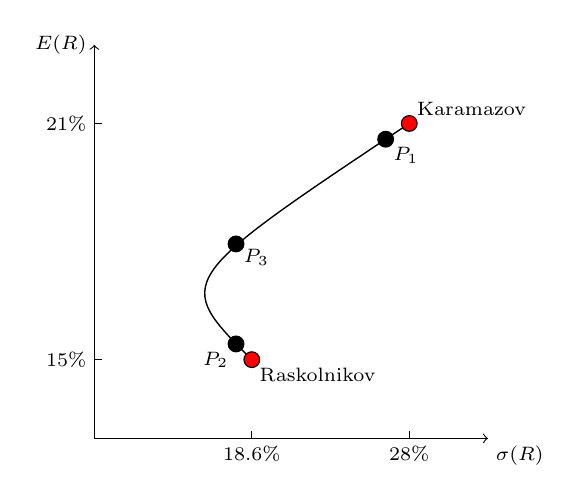
\begin{tikzpicture}
\scriptsize
\draw[->] (0,0) -- (0,5);
\draw[->] (0,0) -- (5,0);
\draw[dashed] (2,0) -- (2,0.1);
\draw[dashed] (0,1) -- (0.1,1);
\draw[dashed] (4,0) -- (4,0.1);
\draw[dashed] (0,4) -- (0.1,4);
\draw[line width=0.5pt] (2, 1) .. controls(1,2) .. (4, 4); % mean-var frontier
\draw[fill=red] (2,1) circle(0.1);
\draw[fill=red] (4,4) circle(0.1);

\draw[fill=black] (1.8,2.47) circle(0.1);
\draw[fill=black] (3.7,3.8) circle(0.1);
\draw[fill=black] (1.8,1.2) circle(0.1);

\draw (5,0) node[below right] {$\sigma(R)$};
\draw (0,5) node[ left] {$E(R)$};

\draw (2,1) node[below right] {Raskolnikov};
\draw (4,4) node[above right] {Karamazov};

\draw (1.8,2.5) node[ below right] {$P_3$};
\draw (1.8,1.2) node[ below left] {$P_2$};
\draw (3.7,3.8) node[below right] {$P_1$};

\draw (2,0) node[below] {18.6\%};
\draw (0,1) node[left] {15\%};
\draw (4,0) node[below] {28\%};
\draw (0,4) node[ left] {21\%};
\end{tikzpicture}
\end{center}
}


%%%%%%%%%%%%%%%%%%  SLIDE  %%%%%%%%%%%%%%%%%%
\frame{\frametitle{\large{\textbf{Mean-Variance Frontier}}}
Once you know the Mean-Variance frontier you can compute the \ul{\textbf{minimum} variance portfolio}, the portfolio that has the minimum risk!
\pause
\begin{center}
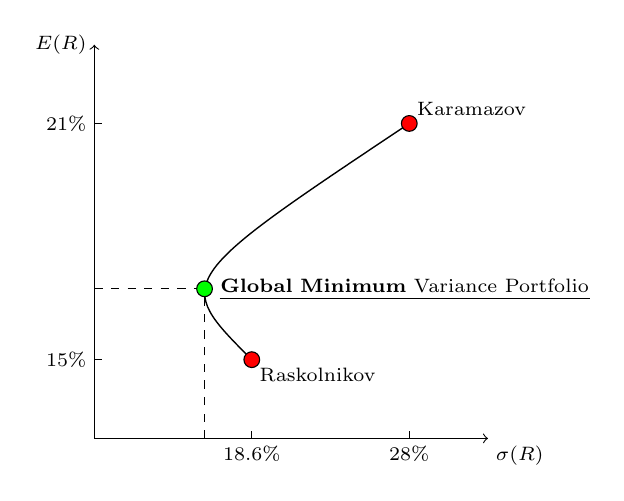
\begin{tikzpicture}
\scriptsize
\draw[->] (0,0) -- (0,5);
\draw[->] (0,0) -- (5,0);
\draw[dashed] (2,0) -- (2,0.1);
\draw[dashed] (0,1) -- (0.1,1);
\draw[dashed] (4,0) -- (4,0.1);
\draw[dashed] (0,4) -- (0.1,4);
\draw[dashed] (0,1.9) -- (1.4,1.9);
\draw[dashed] (1.4,0) -- (1.4,1.9);
\draw[line width=0.5pt] (2, 1) .. controls(1,2) .. (4, 4); % mean-var frontier
\draw[fill=green] (1.4,1.9) circle(0.1);
\draw[fill=red] (2,1) circle(0.1);
\draw[fill=red] (4,4) circle(0.1);
\draw (5,0) node[below right] {$\sigma(R)$};
\draw (0,5) node[ left] {$E(R)$};
\draw (2,1) node[below right] {Raskolnikov};
\draw (4,4) node[above right] {Karamazov};
\draw (1.5,1.9) node[right] {\ul{\textbf{Global Minimum} Variance Portfolio}};
\draw (2,0) node[below] {18.6\%};
\draw (0,1) node[left] {15\%};
\draw (4,0) node[below] {28\%};
\draw (0,4) node[ left] {21\%};
\end{tikzpicture}
\end{center}
}


%%%%%%%%%%%%%%%%%%  SLIDE  %%%%%%%%%%%%%%%%%%
\frame{\frametitle{\large{\textbf{Minimum Variance Portfolio}}}
\bi
\i One way to understand the benefits of diversification is to look at the portfolio that provides the investor with the smallest possible variance: the  \textbf{global minimum-variance portfolio}.
\vv
\i In the case of a two stock portfolio (security 1 and 2), the weights in such a portfolio are given by the following:
\baa
w_1&=&\frac{\sigma_2^2-\rho_{12}\sigma_1\sigma_2}{\sigma_1^2+\sigma_2^2-2\rho_{12}\sigma_1\sigma_2}\\
 w_2&=&1-w_1
\eaa
\ei
}



%%%%%%%%%%%%%%%%%%  SLIDE  %%%%%%%%%%%%%%%%%%

\frame{\frametitle{\large{\textbf{Mean-Variance Frontier}}}
If you were to repeat the above exercise, but instead of using correlation equal to 0.2, you use correlation equal to -1, you obtain the Mean-Variance frontier below.
\begin{center}
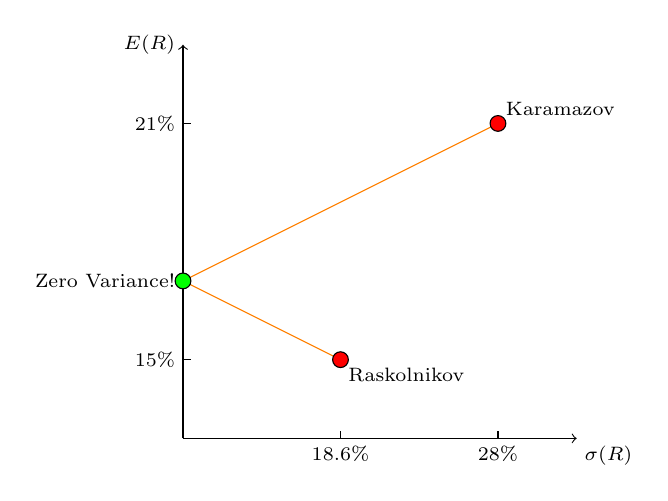
\begin{tikzpicture}
\scriptsize
\draw[->] (0,0) -- (0,5);
\draw[->] (0,0) -- (5,0);
\draw[dashed] (2,0) -- (2,0.1);
\draw[dashed] (0,1) -- (0.1,1);
\draw[dashed] (4,0) -- (4,0.1);
\draw[dashed] (0,4) -- (0.1,4);
%\draw[line width=0.5pt] (2, 1) .. controls(1,2) .. (4, 4); % mean-var frontier for rho=0.2
\draw[orange, -] (0, 2) -- (4, 4); % mean-var frontier for rho=-1
\draw[orange, -] (0, 2) -- (2, 1);  % mean-var frontier for rho=-1
%\draw[blue, -] (2, 1) -- (4, 4);  % mean-var frontier for rho=1
\draw[fill=green] (0,2) circle(0.1);
\draw[fill=red] (2,1) circle(0.1);
\draw[fill=red] (4,4) circle(0.1);
\draw (5,0) node[below right] {$\sigma(R)$};
\draw (0,5) node[ left] {$E(R)$};
\draw (2,1) node[below right] {Raskolnikov};
\draw (4,4) node[above right] {Karamazov};
\draw (0,2) node[left] {Zero Variance!};
\draw (2,0) node[below] {18.6\%};
\draw (0,1) node[left] {15\%};
\draw (4,0) node[below] {28\%};
\draw (0,4) node[ left] {21\%};
\end{tikzpicture}
\end{center}
}


\frame{\frametitle{\large{\textbf{Mean-Variance Frontier}}}
If you were to repeat the above exercise, but with correlation equal to 1, you obtain the following Mean-Variance frontier. There are no gains in diversification! Why?
\begin{center}
\begin{tikzpicture}
\scriptsize
\draw[->] (0,0) -- (0,5);
\draw[->] (0,0) -- (5,0);
\draw[dashed] (2,0) -- (2,0.1);
\draw[dashed] (0,1) -- (0.1,1);
\draw[dashed] (4,0) -- (4,0.1);
\draw[dashed] (0,4) -- (0.1,4);
%\draw[line width=0.5pt] (2, 1) .. controls(1,2) .. (4, 4); % mean-var frontier for rho=0.2
%\draw[red, -] (0, 2) -- (4, 4); % mean-var frontier for rho=-1
%\draw[red, -] (0, 2) -- (2, 1);  % mean-var frontier for rho=-1
\draw[blue, -] (2, 1) -- (4, 4);  % mean-var frontier for rho=1
\draw[fill=red] (2,1) circle(0.1);
\draw[fill=red] (4,4) circle(0.1);
\draw (5,0) node[below right] {$\sigma(R)$};
\draw (0,5) node[ left] {$E(R)$};
\draw (2,1) node[below right] {Raskolnikov};
\draw (4,4) node[above right] {Karamazov};
\draw (2,0) node[below] {18.6\%};
\draw (0,1) node[left] {15\%};
\draw (4,0) node[below] {28\%};
\draw (0,4) node[ left] {21\%};
\end{tikzpicture}
\end{center}
}


\frame{\frametitle{\large{\textbf{Mean-Variance Frontier}}}
Below, the three cases together, where $\rho$ represents the correlation.
\begin{center}
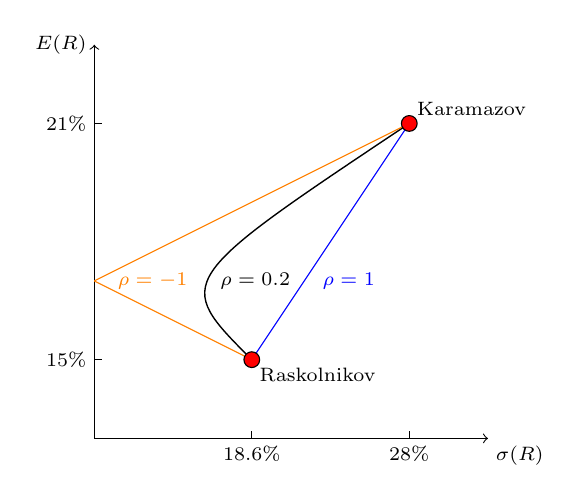
\begin{tikzpicture}
\scriptsize
\draw[->] (0,0) -- (0,5);
\draw[->] (0,0) -- (5,0);
\draw[dashed] (2,0) -- (2,0.1);
\draw[dashed] (0,1) -- (0.1,1);
\draw[dashed] (4,0) -- (4,0.1);
\draw[dashed] (0,4) -- (0.1,4);
\draw[line width=0.5pt] (2, 1) .. controls(1,2) .. (4, 4); % mean-var frontier for rho=0.2
\draw[orange, -] (0, 2) -- (4, 4); % mean-var frontier for rho=-1
\draw[orange, -] (0, 2) -- (2, 1);  % mean-var frontier for rho=-1
\draw[blue, -] (2, 1) -- (4, 4);  % mean-var frontier for rho=1
\draw[fill=red] (2,1) circle(0.1);
\draw[fill=red] (4,4) circle(0.1);
\draw (5,0) node[below right] {$\sigma(R)$};
\draw (0,5) node[ left] {$E(R)$};
\draw (2,1) node[below right] {Raskolnikov};
\draw (4,4) node[above right] {Karamazov};
\draw (0.2,2) node[right] {\color{orange}$\rho=-1$};
\draw (1.5,2) node[right] {$\rho=0.2$};
\draw (2.8,2) node[right] {\color{blue}$\rho=1$};
\draw (2,0) node[below] {18.6\%};
\draw (0,1) node[left] {15\%};
\draw (4,0) node[below] {28\%};
\draw (0,4) node[ left] {21\%};
\end{tikzpicture}
\end{center}
}

\frame{\frametitle{\large{\textbf{Efficiency}}}
Is it better to invest 100\% in Raskolnikov or in Portfolio $P_4$? Why? \pause For the same risk, portfolio $P_{4}$ offers a higher expected return! Always choose $P_{4}$ over Raskolnikov Inc.
\begin{center}
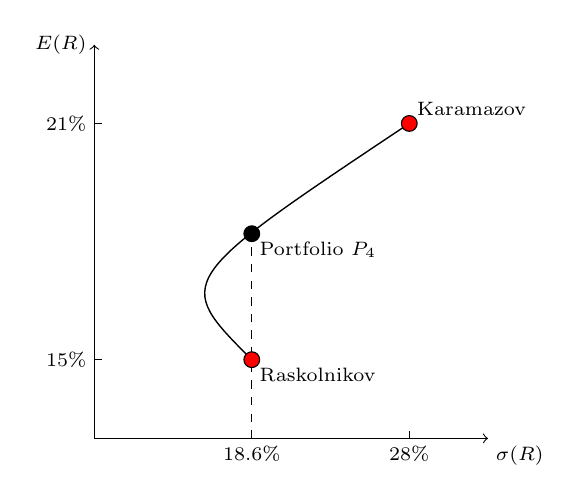
\begin{tikzpicture}
\scriptsize
\draw[->] (0,0) -- (0,5);
\draw[->] (0,0) -- (5,0);
\draw[dashed] (2,0) -- (2,2.6);
\draw[dashed] (0,1) -- (0.1,1);
\draw[dashed] (4,0) -- (4,0.1);
\draw[dashed] (0,4) -- (0.1,4);
\draw[line width=0.5pt] (2, 1) .. controls(1,2) .. (4, 4); % mean-var frontier
\draw[fill=black] (2,2.6) circle(0.1);
\draw[fill=red] (2,1) circle(0.1);
\draw[fill=red] (4,4) circle(0.1);
\draw (5,0) node[below right] {$\sigma(R)$};
\draw (0,5) node[ left] {$E(R)$};
\draw (2,1) node[below right] {Raskolnikov};
\draw (4,4) node[above right] {Karamazov};
\draw (2,2.6) node[below right] {Portfolio $P_4$};
\draw (2,0) node[below] {18.6\%};
\draw (0,1) node[left] {15\%};
\draw (4,0) node[below] {28\%};
\draw (0,4) node[ left] {21\%};
\end{tikzpicture}
\end{center}

}


\frame{\frametitle{\large{\textbf{Efficiency Mean-Variance Frontier}}}
The points of the frontier between above the global minimum variance portfolio are the \textbf{efficient mean-variance frontier} (green line). 
\begin{center}
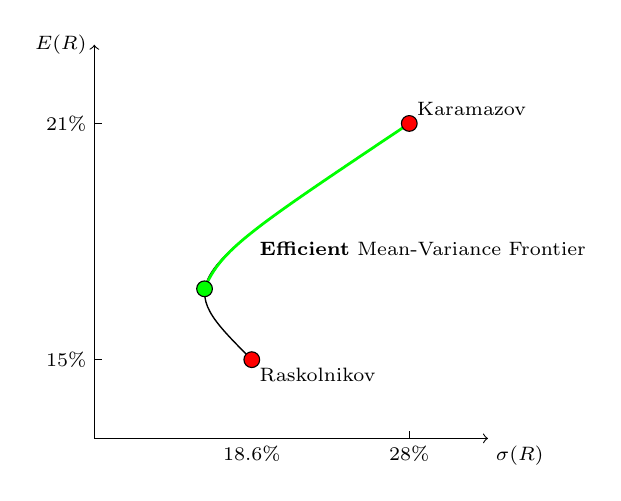
\begin{tikzpicture}
\scriptsize
\draw[->] (0,0) -- (0,5);
\draw[->] (0,0) -- (5,0);
\draw[dashed] (0,1) -- (0.1,1);
\draw[dashed] (4,0) -- (4,0.1);
\draw[dashed] (0,4) -- (0.1,4);
\draw[line width=0.5pt] (2, 1) .. controls(1,2) .. (4, 4); % mean-var frontier
\draw[line width=1pt ,green] (1.4,1.9) .. controls(1.60,2.40) and (2,2.66) .. (4, 4); % efficient mean-var frontier
\draw[fill=green] (1.4,1.9) circle(0.1);
\draw[fill=red] (2,1) circle(0.1);
\draw[fill=red] (4,4) circle(0.1);
\draw (5,0) node[below right] {$\sigma(R)$};
\draw (0,5) node[ left] {$E(R)$};
\draw (2,1) node[below right] {Raskolnikov};
\draw (4,4) node[above right] {Karamazov};
\draw (2,2.6) node[below right] {\textbf{Efficient} Mean-Variance Frontier};
\draw (2,0) node[below] {18.6\%};
\draw (0,1) node[left] {15\%};
\draw (4,0) node[below] {28\%};
\draw (0,4) node[ left] {21\%};
\end{tikzpicture}
\end{center}
}

\frame{\frametitle{\large{\textbf{Risk Preferences}}}
Among the portfolios in the mean-variance frontier, investors choose the one that suits their risk-preferences. Both, $P_{4}$ and $P_{5}$, are in the efficient mean-variance frontier, but $P_{5}$ has a higher $E(R)$ and higher $\sigma(R)$.
\begin{center}
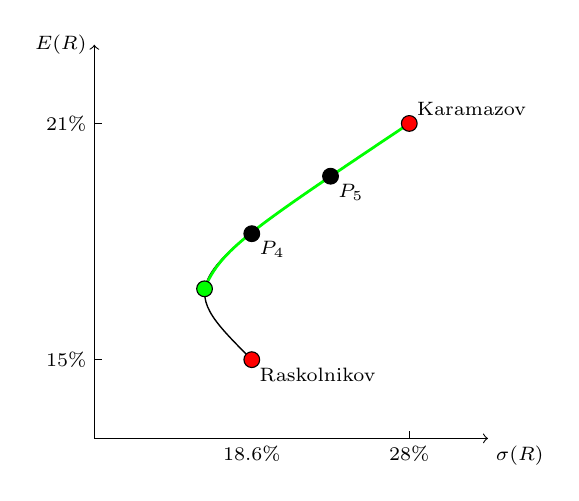
\begin{tikzpicture}
\scriptsize
\draw[->] (0,0) -- (0,5);
\draw[->] (0,0) -- (5,0);
\draw[dashed] (0,1) -- (0.1,1);
\draw[dashed] (4,0) -- (4,0.1);
\draw[dashed] (0,4) -- (0.1,4);
\draw[line width=0.5pt] (2, 1) .. controls(1,2) .. (4, 4); % mean-var frontier
\draw[line width=1pt ,green] (1.4,1.9) .. controls(1.60,2.40) and (2,2.66) .. (4, 4); % efficient mean-var frontier
\draw[fill=green] (1.4,1.9) circle(0.1);
\draw[fill=black] (2,2.6) circle(0.1);
\draw[fill=black] (3,3.33) circle(0.1);
\draw[fill=red] (2,1) circle(0.1);
\draw[fill=red] (4,4) circle(0.1);
\draw (5,0) node[below right] {$\sigma(R)$};
\draw (0,5) node[ left] {$E(R)$};
\draw (2,1) node[below right] {Raskolnikov};
\draw (4,4) node[above right] {Karamazov};
\draw (2,2.6) node[below right] {$P_{4}$};
\draw (3,3.33) node[below right] {$P_{5}$};
\draw (2,0) node[below] {18.6\%};
\draw (0,1) node[left] {15\%};
\draw (4,0) node[below] {28\%};
\draw (0,4) node[ left] {21\%};
\end{tikzpicture}
\end{center}
}


\frame{\frametitle{\large{\textbf{Summary}}}
\bi
\i Given a portfolio of assets, you can always compute the mean-variance frontier;
\vv
\i The shape of the mean-variance frontier depends on the correlation between securities;
\vv 
\i There is an efficient part of the mean-variance frontier, investors should always choose portfolios that lie on the efficient part;
\vv
\i Risk aversion defines where in the efficient mean-variance frontier investors want to be (more on this next class);
\ei
}



%%%%%%%%%%%%%%%%%%  SLIDE  %%%%%%%%%%%%%%%%%%
%\frame{\frametitle{\large{\textbf{title?}}}
%\bi
%\i 
%\vv
%\ei
%}

\newcounter{finalframe}
\setcounter{finalframe}{\value{framenumber}}

\setcounter{framenumber}{\value{finalframe}}
\end{document}



